%% 
%% This is file, `info_merkzettel_wichtig.tex',
%% generated with the extract package.
%% 
%% Generated on :  2022/11/30,0:59
%% From source  :  info_merkzettel.tex
%% Using options:  active,generate=info_merkzettel_wichtig,extract-env=mzImportant,copydocumentclass=false,
%% 
    \documentclass[uniLeipzig]{merkzettel}
  

\begin{document}

\begin{mzImportant}
  \mzGraphic{
    \begin{tblr}{
      cells = {c},
      cell{1}{1} = {c=2}{},
      cell{2}{3} = {r=2}{r},
      cell{4}{3} = {r=2}{r},
      cell{6}{3} = {r=2}{r},
      cell{8}{3} = {r=2}{r},
      cell{10}{3} = {r},
      cell{11}{3} = {r=2}{r},
      cell{13}{3} = {r=2}{r},
      cell{15}{3} = {r=3}{r},
      vline{2} = {2-17}{},
      hline{1-2,18} = {-}{},
        }
      \textbf{Äquivalente Formeln $\boldsymbol{\Leftrightarrow}$}               &                                                 & Bezeichnung \\
      $A \land B$                                & $B \land A$                                     & \index{Logische Kommutativität}Kommutativ  \\
      $A \lor B$                                 & $B \lor A$                                      &             \\
      $A \land (B \land C)$                      & $(A \land B) \land C$                           & \index{Logische Assoziativität}Assoziativ  \\
      $A \lor (B \lor C)$                        & $(A \lor B) \lor C$                             &             \\
      $A \land (B \lor C)$                       & $(A \land B) \lor (A \land C)$                  & \index{Logische Distributivität}Distributiv \\
      $A \lor (B \land C)$                       & $(A \lor B) \land (A \lor C)$                   &             \\
      $A \land A$                                & $A$                                             & \index{Idempotenz}Idempotenz  \\
      $A \lor A$                                 & $A$                                             &             \\
      $\neg \neg A$                              & $A$                                             & \index{Involution}Involution  \\
      $\neg (A \land B)$                         & $\neg A \boldsymbol{\lor} \neg B$  & \index{\textsc{De-Morgan}}\textsc{De-Morgan}   \\
      $\neg (A \lor B)$                          & $\neg A \boldsymbol{\land} \neg B$ &             \\
      $A \land (\mathbf{A} \lor B)$ & $A$                                             & \index{Absoption}Absorption  \\
      $A \lor (\mathbf{A} \land B)$ & $A$                                             &             \\
      $A \Rightarrow B$                          & $\mathbf{\neg A} \lor B$           & \index{Elimination}Elimination \\
      $\neg (A \Rightarrow B)$                   & $A \land \neg B$                                &             \\
      $A \Leftrightarrow B$                      & $(A \Rightarrow B) \land (B \Rightarrow A)$     &
    \end{tblr}
  }
\end{mzImportant}

\begin{mzImportant}
          \begin{description}
            \item [$\mathcal{A} \Rightarrow \mathcal{B}$] ,,$\mathcal{A}$ hinreichend``
                  \index{Hinreichende Bedingung}
            \item [$\mathcal{B} \Rightarrow \mathcal{A}$] ,,$\mathcal{A}$ notwendig``
                  \index{Notwendige Bedingung}
          \end{description}
        
\end{mzImportant}

\begin{mzImportant}
  \mzGraphic{
    \begin{tblr}{
      cells = {c},
      cell{1}{1} = {c=2}{},
      cell{2}{3} = {r=2}{r},
      cell{4}{3} = {r=2}{r},
      cell{6}{3} = {r=2}{r},
      cell{8}{3} = {r=2}{r},
      cell{10}{3} = {r},
      cell{11}{3} = {r=2}{r},
      cell{13}{3} = {r=2}{r},
      cell{15}{3} = {r=3}{r},
      vline{2} = {2-17}{},
      hline{1-2,18} = {-}{},
        }
      \textbf{Äquivalente Formeln $\boldsymbol{\Leftrightarrow}$}               &                                                 & Bezeichnung \\
      $A \land B$                                & $B \land A$                                     & \index{Logische Kommutativität}Kommutativ  \\
      $A \lor B$                                 & $B \lor A$                                      &             \\
      $A \land (B \land C)$                      & $(A \land B) \land C$                           & \index{Logische Assoziativität}Assoziativ  \\
      $A \lor (B \lor C)$                        & $(A \lor B) \lor C$                             &             \\
      $A \land (B \lor C)$                       & $(A \land B) \lor (A \land C)$                  & \index{Logische Distributivität}Distributiv \\
      $A \lor (B \land C)$                       & $(A \lor B) \land (A \lor C)$                   &             \\
      $A \land A$                                & $A$                                             & \index{Idempotenz}Idempotenz  \\
      $A \lor A$                                 & $A$                                             &             \\
      $\neg \neg A$                              & $A$                                             & \index{Involution}Involution  \\
      $\neg (A \land B)$                         & $\neg A \boldsymbol{\lor} \neg B$  & \index{\textsc{De-Morgan}}\textsc{De-Morgan}   \\
      $\neg (A \lor B)$                          & $\neg A \boldsymbol{\land} \neg B$ &             \\
      $A \land (\mathbf{A} \lor B)$ & $A$                                             & \index{Absoption}Absorption  \\
      $A \lor (\mathbf{A} \land B)$ & $A$                                             &             \\
      $A \Rightarrow B$                          & $\mathbf{\neg A} \lor B$           & \index{Elimination}Elimination \\
      $\neg (A \Rightarrow B)$                   & $A \land \neg B$                                &             \\
      $A \Leftrightarrow B$                      & $(A \Rightarrow B) \land (B \Rightarrow A)$     &
    \end{tblr}
  }
\end{mzImportant}

\begin{mzImportant}
          \begin{description}
            \item [$\mathcal{A} \Rightarrow \mathcal{B}$] ,,$\mathcal{A}$ hinreichend``
                  \index{Hinreichende Bedingung}
            \item [$\mathcal{B} \Rightarrow \mathcal{A}$] ,,$\mathcal{A}$ notwendig``
                  \index{Notwendige Bedingung}
          \end{description}
        
\end{mzImportant}

\begin{mzImportant}
  \mzGraphic{
    \begin{tblr}{
      cells = {c},
      cell{1}{1} = {c=2}{},
      cell{2}{3} = {r=2}{r},
      cell{4}{3} = {r=2}{r},
      cell{6}{3} = {r=2}{r},
      cell{8}{3} = {r=2}{r},
      cell{10}{3} = {r},
      cell{11}{3} = {r=2}{r},
      cell{13}{3} = {r=2}{r},
      cell{15}{3} = {r=3}{r},
      vline{2} = {2-17}{},
      hline{1-2,18} = {-}{},
        }
      \textbf{Äquivalente Formeln $\boldsymbol{\Leftrightarrow}$}               &                                                 & Bezeichnung \\
      $A \land B$                                & $B \land A$                                     & \index{Logische Kommutativität}Kommutativ  \\
      $A \lor B$                                 & $B \lor A$                                      &             \\
      $A \land (B \land C)$                      & $(A \land B) \land C$                           & \index{Logische Assoziativität}Assoziativ  \\
      $A \lor (B \lor C)$                        & $(A \lor B) \lor C$                             &             \\
      $A \land (B \lor C)$                       & $(A \land B) \lor (A \land C)$                  & \index{Logische Distributivität}Distributiv \\
      $A \lor (B \land C)$                       & $(A \lor B) \land (A \lor C)$                   &             \\
      $A \land A$                                & $A$                                             & \index{Idempotenz}Idempotenz  \\
      $A \lor A$                                 & $A$                                             &             \\
      $\neg \neg A$                              & $A$                                             & \index{Involution}Involution  \\
      $\neg (A \land B)$                         & $\neg A \boldsymbol{\lor} \neg B$  & \index{\textsc{De-Morgan}}\textsc{De-Morgan}   \\
      $\neg (A \lor B)$                          & $\neg A \boldsymbol{\land} \neg B$ &             \\
      $A \land (\mathbf{A} \lor B)$ & $A$                                             & \index{Absoption}Absorption  \\
      $A \lor (\mathbf{A} \land B)$ & $A$                                             &             \\
      $A \Rightarrow B$                          & $\mathbf{\neg A} \lor B$           & \index{Elimination}Elimination \\
      $\neg (A \Rightarrow B)$                   & $A \land \neg B$                                &             \\
      $A \Leftrightarrow B$                      & $(A \Rightarrow B) \land (B \Rightarrow A)$     &
    \end{tblr}
  }
\end{mzImportant}

\begin{mzImportant}
  \index{Gro\ss-O-Notation}
  \paragraph{Gro\ss-O-Notation}
  Kosten $C_f(n)$ mit $g: \mathbb{N} \rightarrow \mathbb{R} \exists c > 0 \exists n_0 > 0 \forall n \geq n_0$

  \begin{description}
    \item [Untere Schranke] $\boldsymbol{\Omega} (f)$ \\
          \index{Untere Schranke Komplexität}
          $C_f(n) \boldsymbol{\geq} c * g(n)$

    \item [Obere Schranke] $\boldsymbol{O}(f)$ \\
          \index{Obere Schranke Komplexität}
          $C_f(n) \boldsymbol{\leq} c * g(n)$

    \item [Exakte Schranke] $\boldsymbol{\Theta} (f)$ \\
          \index{Exakte Schranke Komplexität}
          $C_f(n) \in \Omega (f) \cap O(f)$ \\
          Polynom $k$ten Grades $\in \Theta (n^k)$
  \end{description}

  (Beweis: $g$ und $c$ finden)
\end{mzImportant}

\begin{mzImportant}
  \begin{description}
    \item [Elementare Operationen, Kontrollstr.]
          $\mathbf{\in O(1)}$

    \item [Schleifen]
          $\in$ $i$ Wiederholungen $\boldsymbol{*}$ $O(f)$ teuerste Operation

    \item [Abfolge]
          $O(g)$ nach $O(f)$ $\in O(\boldsymbol{\max} (f;g))$

    \item [Rekursion]
          $\in$ $k$ Aufrufe $\boldsymbol{*}$ $O(f)$ teuerste Operation
  \end{description}
\end{mzImportant}

\begin{mzImportant}
  \index{Mastertheorem}
  \paragraph{Mastertheorem} $a \geq 1$, $b > 1$, $\Theta \geq 0$

  \begin{gather*}
    T(n) = a * T( \frac{n}{b} ) + \Theta (n^k) \\
    \Rightarrow \begin{cases}
      \Theta ( n^k ) \quad          & a < b^k \\
      \Theta ( n^k \log n ) \quad   & a = b^k \\
      \Theta ( n^{\log_b a} ) \quad & a > b^k
    \end{cases}
  \end{gather*}
\end{mzImportant}

\begin{mzImportant}
  \paragraph{Skip}
  \index{Skip-Liste}

  \mzGraphic{
    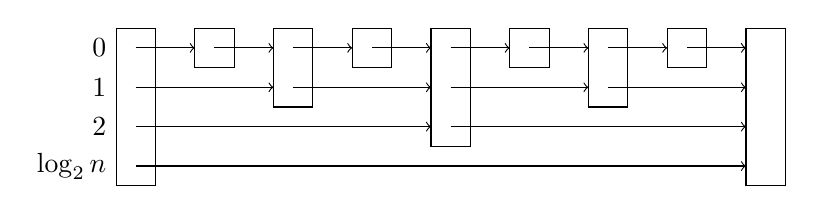
\begin{tikzpicture}[scale=.5,yscale=-1]
      \draw
      (-2,0) rectangle (-1,4)

      (0,0) rectangle (1,1)
      (2,0) rectangle (3,2)
      (4,0) rectangle (5,1)
      (6,0) rectangle (7,3)
      (8,0) rectangle (9,1)

      (10,0) rectangle (11,2)
      (12,0) rectangle (13,1)

      (14,0) rectangle (15,4);

      \draw[->] (-1.5,.5) -- (0,.5);
      \draw[->] (0.5,.5) -- (2,.5);
      \draw[->] (2.5,.5) -- (4,.5);
      \draw[->] (4.5,.5) -- (6,.5);
      \draw[->] (6.5,.5) -- (8,.5);

      \draw[->] (8.5,.5) -- (10,.5);
      \draw[->] (10.5,.5) -- (12,.5);
      \draw[->] (12.5,.5) -- (14,.5);

      \draw[->] (-1.5,1.5) -- (2,1.5);
      \draw[->] (2.5,1.5) -- (6,1.5);
      \draw[->] (6.5,1.5) -- (10,1.5);
      \draw[->] (10.5,1.5) -- (14,1.5);

      \draw[->] (-1.5,2.5) -- (6,2.5);
      \draw[->] (6.5,2.5) -- (14,2.5);

      \draw[->] (-1.5,3.5) -- (14,3.5);

      \draw
      (-2,.5) node[left] {$0$}
      (-2,1.5) node[left] {$1$}
      (-2,2.5) node[left] {$2$}
      (-2,3.5) node[left] {$\floor{\log_2 n}$};
    \end{tikzpicture}
  }

  \begin{itemize}
    \item Zeiger auf Ebene $i$ zeigt zu nächstem $2^i$ Element
    \item Suchen $\in O(\log n)$
  \end{itemize}

  \begin{description}
    \item [(Perfekt)]
          \index{Perfekte Skip-Liste}
          Einfügen, Löschen $\mathbf{\in O(n)}$ (Vollst. Reorga.)

    \item [Randomisiert]
          \index{Randomisierte Skip-Liste}
          Höhe zufällig (keine vollst. Reorga.) \\
          $P(h) = \frac{1}{2^{h + 1}}$: Einfügen, Löschen $\mathbf{\in O(\log n)}$
  \end{description}
\end{mzImportant}

\begin{mzImportant}
  \paragraph{Sortierproblem}
  \index{Sortierproblem}

  \begin{description}
    \item[Gegeben] (endliche) Folge von Schlüsseln (von Daten) $(K_i)_{i \in I}$
    \item[Gesucht] Bijektive Abbildung $\pi: I \rightarrow I$ (Permutation), sodass $K_{\pi(i)} \leq K_{\pi(i + 1)} \quad \forall i \in I$
  \end{description}
\end{mzImportant}

\begin{mzImportant}
  \begin{description}
    \item [Ordnung] \emph{Allgemein} vs. \emph{speziell}: Ordnung wird nur über Schlüsselvergleiche hergestellt
          \index{Allgemeine Suche}
          \index{Spezielle Suche}
    \item [Relation] \emph{Stabil} vs. \emph{instabil}: Vorherig relative Reihenfolge bleibt erhalten
          \index{Stabile Suche}
          \index{Instabile Suche}
    \item [Speicher] \emph{In situ} vs. \emph{ex situ}: Zusätzlicher Speicher notwendig
          \index{In situ Suche}
          \index{Ex situ Suche}
    \item [Lokal] \emph{Intern} vs. \emph{extern}: Alles im RAM oder Mischung vorsortierter externer Teilfolgen
          \index{Interne Suche}
          \index{Externe Suche}
  \end{description}
\end{mzImportant}

\begin{mzImportant}
  \begin{description}
    \item [Anzahl der Inversionen]
          \index{Anzahl der Inversionen}
          Anzahl kleinerer Nachfolger für jedes Element:
          \begin{gather*}
            \text{inv} (L) := |\{ (i,j) \mid \\
            0 \leq i < j \leq n - 1, \\
            L[i] \geq L[j] \}|
          \end{gather*}

    \item [Anzahl der Runs]
          \index{Run}
          Ein \emph{Run} ist eine sortierte Teilliste, die nicht nach links oder rechts verlängert werden kann.
          Die Anzahl der Runs ist:
          \begin{gather*}
            \text{runs} (L) := |\{ i \mid \\
            0 \leq i < n - 1, \\
            L[i + 1] < L[i]  \}| \mathbf{+ 1}
          \end{gather*}

    \item [Längster Run]
          \index{Längster Run}
          Anzahl der Elemente der längsten sortierten Teilliste:
          \begin{gather*}
            \text{las} (L) := \max \{ r.\text{len} \mid \\
            r \text{ ist Run in } L \} \\
            \text{rem} (L) := L.\text{len} - \text{las} (L)
          \end{gather*}
  \end{description}
\end{mzImportant}

\begin{mzImportant}
  Jedes allgemeine Sortierverfahren benötigt im Worst- und Average-case Schlüsselvergleiche von mindestens:

  $$\Omega (n \log n)$$
\end{mzImportant}

\begin{mzImportant}
  \paragraph{Lexikographische Ordnung $\mathbf{\leq}$}
  \index{Lexikographische Ordnung}
  Sei $A = \{ a_1, \dots, a_n \}$ ein Alphabet, dass sich mit gegebener Ordnung $a_1 < \cdots < a_n$ wie folgt auf dem Lexikon $A* = \bigcup_{n \in \mathbb{N}_0} A^n$ fortsetzt:
  \begin{align*}
                    & v = (v_1, \dots, v_p) \leq w = (w_1, \dots, w_q)   \\
    \Leftrightarrow & \forall 1 \leq i \leq p: v_i = w_i \quad p \leq q  \\
    \lor            & \forall 1 \leq j \leq i: v_j = w_j \quad v_i < w_i
  \end{align*}

  \paragraph{Fachverteilen}
  \index{Fachverteilen}
  Sortieren von $n$ $k$-Tupeln in $k$ Schritten: Sortieren nach letztem Element, vorletzem usw.
\end{mzImportant}

\begin{mzImportant}
  % TODO: Merge Shell sort cells and add this text:
  % Abhängig von Sprunggrö\ss en $h_i$: $O(n \log n)$, $O(n^\frac{3}{2})$ bis $O(n^2)$ (h_i = 1)
  \mzGraphic{
    \begin{tblr}{
      row{2} = {c},
      row{12} = {c},
      cell{1}{1} = {r=2}{},
      cell{1}{2} = {r=2}{c},
      cell{1}{3} = {r=2}{c},
      cell{1}{4} = {c=3}{c},
      cell{1}{7} = {c=3}{c},
      cell{1}{10} = {r=2}{r},
      cell{3}{2} = {c},
      cell{3}{3} = {c},
      cell{3}{4} = {c},
      cell{3}{5} = {c},
      cell{3}{6} = {c},
      cell{3}{7} = {c},
      cell{3}{8} = {c},
      cell{3}{9} = {c},
      cell{3}{10} = {r=3}{c},
      cell{4}{2} = {c},
      cell{4}{3} = {c},
      cell{4}{4} = {c},
      cell{4}{5} = {c},
      cell{4}{6} = {c},
      cell{4}{7} = {c},
      cell{4}{8} = {c},
      cell{4}{9} = {c},
      cell{5}{2} = {c},
      cell{5}{3} = {c},
      cell{5}{4} = {c},
      cell{5}{5} = {c},
      cell{5}{6} = {c},
      cell{5}{7} = {c},
      cell{5}{8} = {c},
      cell{5}{9} = {c},
      cell{6}{4} = {c=2}{c},
      cell{6}{6} = {c=2}{c},
      cell{6}{8} = {c=2}{c},
      cell{7}{2} = {c},
      cell{7}{3} = {c},
      cell{7}{4} = {c=2}{c},
      cell{7}{6} = {c=2}{c},
      cell{7}{8} = {c=2}{c},
      cell{7}{10} = {r=5}{c},
      cell{8}{2} = {c},
      cell{8}{3} = {c},
      cell{8}{4} = {c=2}{c},
      cell{8}{6} = {c=2}{c},
      cell{8}{8} = {c=2}{c},
      cell{9}{2} = {c},
      cell{9}{3} = {c},
      cell{9}{4} = {c=2}{c},
      cell{9}{6} = {c=2}{c},
      cell{9}{8} = {c=2}{c},
      cell{10}{2} = {c},
      cell{10}{3} = {c},
      cell{10}{4} = {c=2}{c},
      cell{10}{6} = {c=2}{c},
      cell{10}{8} = {c=2}{c},
      cell{11}{2} = {c},
      cell{11}{3} = {c},
      cell{11}{4} = {c=2}{c},
      cell{11}{6} = {c=2}{c},
      cell{11}{8} = {c=2}{c},
      cell{12}{1} = {c=10}{},
      cell{13}{2} = {c},
      cell{13}{3} = {c},
      cell{13}{4} = {c=2}{c},
      cell{13}{6} = {c=2}{c},
      cell{13}{8} = {c=2}{c},
      cell{13}{10} = {r},
      hline{1,3,6-7,12-14} = {-}{},
        }
      \textbf{Algo.} & \textbf{Stabil} & \textbf{Mem.} & \textbf{Schlüsselvergleiche} &  &  & \textbf{Satzbewegungen} &  &  & \\

      &  &  & $C_B$ & $C_A$ & $C_W$ & $M_B$ & $M_A$ & $M_W$ & \\

      Selection & \ding{55} & $1$ & $\frac{n (n - 1)}{2}$ & $\frac{n (n - 1)}{2}$ & $\frac{n (n - 1)}{2}$ & $3 (n - 1)$ & $3 (n - 1)$ & $3 (n -1)$ & \begin{sideways}$O(n^2)$\end{sideways}\\

      Insertion & \ding{51} & $1$ & $n - 1$ & $\overset{n \rightarrow \infty}{\approx} \frac{n (n - 1)}{4} + n - \ln n$ & $\frac{n (n - 1)}{2}$ & $2 (n - 1)$ & $\frac{n^2 + 3n - 4}{4} + n - 1$ & $\frac{n^2 + 3n - 4}{2}$ & \\

      Bubble & \ding{51} & $1$ & $\frac{n (n - 1)}{2}$ & $\frac{n (n - 1)}{2}$ & $\frac{n (n - 1)}{2}$ & $0$ & $\frac{3n (n - 1)}{4}$ & $\frac{3n (n - 1)}{2}$ & \\

      &  &  & \textbf{Best-case} &  & \textbf{Average-case} &  & \textbf{Worst-case} &  & \\

      Shell & \ding{55} & $1$ & - &  & - &  & - &  & \begin{sideways}$O(n \log n)$\end{sideways}\\

      Quick & \ding{55} & $\log n$ & $n \log n$ & & $n \log n$ & & $n^2$ & & \\

      Turnier & \ding{55} & $2n - 1$ & $n \log n$ & & $n \log n$ & & $n \log n$ & & \\

      Heap & \ding{55} & $1$ & $n \log n$ & & $n \log n$ &  & $n \log n$ &  & \\

      Merge & \ding{51} & $n$ & $n \log n$ &  & $n \log n$ &  & $n \log n$ &  & \\

      \textbf{Untere Schranke $\Omega (n \log n)$ für allgemeine Sortierverfahren} & & & & & & & & & \\

      Distribution & \ding{51} & $n$ & $n$ &  & $n$ &  & $n \log n$, $n^2$ &  & $O(n)$
    \end{tblr}
  }
\end{mzImportant}

\begin{mzImportant}
  \index{Gro\ss-O-Notation}
  \paragraph{Gro\ss-O-Notation}
  Kosten $C_f(n)$ mit $g: \mathbb{N} \rightarrow \mathbb{R} \exists c > 0 \exists n_0 > 0 \forall n \geq n_0$

  \begin{description}
    \item [Untere Schranke] $\boldsymbol{\Omega} (f)$ \\
          \index{Untere Schranke Komplexität}
          $C_f(n) \boldsymbol{\geq} c * g(n)$

    \item [Obere Schranke] $\boldsymbol{O}(f)$ \\
          \index{Obere Schranke Komplexität}
          $C_f(n) \boldsymbol{\leq} c * g(n)$

    \item [Exakte Schranke] $\boldsymbol{\Theta} (f)$ \\
          \index{Exakte Schranke Komplexität}
          $C_f(n) \in \Omega (f) \cap O(f)$ \\
          Polynom $k$ten Grades $\in \Theta (n^k)$
  \end{description}

  (Beweis: $g$ und $c$ finden)
\end{mzImportant}

\begin{mzImportant}
  \begin{description}
    \item [Elementare Operationen, Kontrollstr.]
          $\mathbf{\in O(1)}$

    \item [Schleifen]
          $\in$ $i$ Wiederholungen $\boldsymbol{*}$ $O(f)$ teuerste Operation

    \item [Abfolge]
          $O(g)$ nach $O(f)$ $\in O(\boldsymbol{\max} (f;g))$

    \item [Rekursion]
          $\in$ $k$ Aufrufe $\boldsymbol{*}$ $O(f)$ teuerste Operation
  \end{description}
\end{mzImportant}

\begin{mzImportant}
  \index{Mastertheorem}
  \paragraph{Mastertheorem} $a \geq 1$, $b > 1$, $\Theta \geq 0$

  \begin{gather*}
    T(n) = a * T( \frac{n}{b} ) + \Theta (n^k) \\
    \Rightarrow \begin{cases}
      \Theta ( n^k ) \quad          & a < b^k \\
      \Theta ( n^k \log n ) \quad   & a = b^k \\
      \Theta ( n^{\log_b a} ) \quad & a > b^k
    \end{cases}
  \end{gather*}
\end{mzImportant}

\begin{mzImportant}
  \paragraph{Skip}
  \index{Skip-Liste}

  \mzGraphic{
    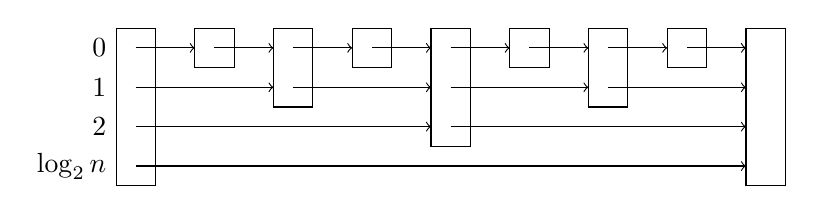
\begin{tikzpicture}[scale=.5,yscale=-1]
      \draw
      (-2,0) rectangle (-1,4)

      (0,0) rectangle (1,1)
      (2,0) rectangle (3,2)
      (4,0) rectangle (5,1)
      (6,0) rectangle (7,3)
      (8,0) rectangle (9,1)

      (10,0) rectangle (11,2)
      (12,0) rectangle (13,1)

      (14,0) rectangle (15,4);

      \draw[->] (-1.5,.5) -- (0,.5);
      \draw[->] (0.5,.5) -- (2,.5);
      \draw[->] (2.5,.5) -- (4,.5);
      \draw[->] (4.5,.5) -- (6,.5);
      \draw[->] (6.5,.5) -- (8,.5);

      \draw[->] (8.5,.5) -- (10,.5);
      \draw[->] (10.5,.5) -- (12,.5);
      \draw[->] (12.5,.5) -- (14,.5);

      \draw[->] (-1.5,1.5) -- (2,1.5);
      \draw[->] (2.5,1.5) -- (6,1.5);
      \draw[->] (6.5,1.5) -- (10,1.5);
      \draw[->] (10.5,1.5) -- (14,1.5);

      \draw[->] (-1.5,2.5) -- (6,2.5);
      \draw[->] (6.5,2.5) -- (14,2.5);

      \draw[->] (-1.5,3.5) -- (14,3.5);

      \draw
      (-2,.5) node[left] {$0$}
      (-2,1.5) node[left] {$1$}
      (-2,2.5) node[left] {$2$}
      (-2,3.5) node[left] {$\floor{\log_2 n}$};
    \end{tikzpicture}
  }

  \begin{itemize}
    \item Zeiger auf Ebene $i$ zeigt zu nächstem $2^i$ Element
    \item Suchen $\in O(\log n)$
  \end{itemize}

  \begin{description}
    \item [(Perfekt)]
          \index{Perfekte Skip-Liste}
          Einfügen, Löschen $\mathbf{\in O(n)}$ (Vollst. Reorga.)

    \item [Randomisiert]
          \index{Randomisierte Skip-Liste}
          Höhe zufällig (keine vollst. Reorga.) \\
          $P(h) = \frac{1}{2^{h + 1}}$: Einfügen, Löschen $\mathbf{\in O(\log n)}$
  \end{description}
\end{mzImportant}

\begin{mzImportant}
  \paragraph{Sortierproblem}
  \index{Sortierproblem}

  \begin{description}
    \item[Gegeben] (endliche) Folge von Schlüsseln (von Daten) $(K_i)_{i \in I}$
    \item[Gesucht] Bijektive Abbildung $\pi: I \rightarrow I$ (Permutation), sodass $K_{\pi(i)} \leq K_{\pi(i + 1)} \quad \forall i \in I$
  \end{description}
\end{mzImportant}

\begin{mzImportant}
  \begin{description}
    \item [Ordnung] \emph{Allgemein} vs. \emph{speziell}: Ordnung wird nur über Schlüsselvergleiche hergestellt
          \index{Allgemeine Suche}
          \index{Spezielle Suche}
    \item [Relation] \emph{Stabil} vs. \emph{instabil}: Vorherig relative Reihenfolge bleibt erhalten
          \index{Stabile Suche}
          \index{Instabile Suche}
    \item [Speicher] \emph{In situ} vs. \emph{ex situ}: Zusätzlicher Speicher notwendig
          \index{In situ Suche}
          \index{Ex situ Suche}
    \item [Lokal] \emph{Intern} vs. \emph{extern}: Alles im RAM oder Mischung vorsortierter externer Teilfolgen
          \index{Interne Suche}
          \index{Externe Suche}
  \end{description}
\end{mzImportant}

\begin{mzImportant}
  \begin{description}
    \item [Anzahl der Inversionen]
          \index{Anzahl der Inversionen}
          Anzahl kleinerer Nachfolger für jedes Element:
          \begin{gather*}
            \text{inv} (L) := |\{ (i,j) \mid \\
            0 \leq i < j \leq n - 1, \\
            L[i] \geq L[j] \}|
          \end{gather*}

    \item [Anzahl der Runs]
          \index{Run}
          Ein \emph{Run} ist eine sortierte Teilliste, die nicht nach links oder rechts verlängert werden kann.
          Die Anzahl der Runs ist:
          \begin{gather*}
            \text{runs} (L) := |\{ i \mid \\
            0 \leq i < n - 1, \\
            L[i + 1] < L[i]  \}| \mathbf{+ 1}
          \end{gather*}

    \item [Längster Run]
          \index{Längster Run}
          Anzahl der Elemente der längsten sortierten Teilliste:
          \begin{gather*}
            \text{las} (L) := \max \{ r.\text{len} \mid \\
            r \text{ ist Run in } L \} \\
            \text{rem} (L) := L.\text{len} - \text{las} (L)
          \end{gather*}
  \end{description}
\end{mzImportant}

\begin{mzImportant}
  Jedes allgemeine Sortierverfahren benötigt im Worst- und Average-case Schlüsselvergleiche von mindestens:

  $$\Omega (n \log n)$$
\end{mzImportant}

\begin{mzImportant}
  \paragraph{Lexikographische Ordnung $\mathbf{\leq}$}
  \index{Lexikographische Ordnung}
  Sei $A = \{ a_1, \dots, a_n \}$ ein Alphabet, dass sich mit gegebener Ordnung $a_1 < \cdots < a_n$ wie folgt auf dem Lexikon $A* = \bigcup_{n \in \mathbb{N}_0} A^n$ fortsetzt:
  \begin{align*}
                    & v = (v_1, \dots, v_p) \leq w = (w_1, \dots, w_q)   \\
    \Leftrightarrow & \forall 1 \leq i \leq p: v_i = w_i \quad p \leq q  \\
    \lor            & \forall 1 \leq j \leq i: v_j = w_j \quad v_i < w_i
  \end{align*}

  \paragraph{Fachverteilen}
  \index{Fachverteilen}
  Sortieren von $n$ $k$-Tupeln in $k$ Schritten: Sortieren nach letztem Element, vorletzem usw.
\end{mzImportant}

\begin{mzImportant}
  % TODO: Merge Shell sort cells and add this text:
  % Abhängig von Sprunggrö\ss en $h_i$: $O(n \log n)$, $O(n^\frac{3}{2})$ bis $O(n^2)$ (h_i = 1)
  \mzGraphic{
    \begin{tblr}{
      row{2} = {c},
      row{12} = {c},
      cell{1}{1} = {r=2}{},
      cell{1}{2} = {r=2}{c},
      cell{1}{3} = {r=2}{c},
      cell{1}{4} = {c=3}{c},
      cell{1}{7} = {c=3}{c},
      cell{1}{10} = {r=2}{r},
      cell{3}{2} = {c},
      cell{3}{3} = {c},
      cell{3}{4} = {c},
      cell{3}{5} = {c},
      cell{3}{6} = {c},
      cell{3}{7} = {c},
      cell{3}{8} = {c},
      cell{3}{9} = {c},
      cell{3}{10} = {r=3}{c},
      cell{4}{2} = {c},
      cell{4}{3} = {c},
      cell{4}{4} = {c},
      cell{4}{5} = {c},
      cell{4}{6} = {c},
      cell{4}{7} = {c},
      cell{4}{8} = {c},
      cell{4}{9} = {c},
      cell{5}{2} = {c},
      cell{5}{3} = {c},
      cell{5}{4} = {c},
      cell{5}{5} = {c},
      cell{5}{6} = {c},
      cell{5}{7} = {c},
      cell{5}{8} = {c},
      cell{5}{9} = {c},
      cell{6}{4} = {c=2}{c},
      cell{6}{6} = {c=2}{c},
      cell{6}{8} = {c=2}{c},
      cell{7}{2} = {c},
      cell{7}{3} = {c},
      cell{7}{4} = {c=2}{c},
      cell{7}{6} = {c=2}{c},
      cell{7}{8} = {c=2}{c},
      cell{7}{10} = {r=5}{c},
      cell{8}{2} = {c},
      cell{8}{3} = {c},
      cell{8}{4} = {c=2}{c},
      cell{8}{6} = {c=2}{c},
      cell{8}{8} = {c=2}{c},
      cell{9}{2} = {c},
      cell{9}{3} = {c},
      cell{9}{4} = {c=2}{c},
      cell{9}{6} = {c=2}{c},
      cell{9}{8} = {c=2}{c},
      cell{10}{2} = {c},
      cell{10}{3} = {c},
      cell{10}{4} = {c=2}{c},
      cell{10}{6} = {c=2}{c},
      cell{10}{8} = {c=2}{c},
      cell{11}{2} = {c},
      cell{11}{3} = {c},
      cell{11}{4} = {c=2}{c},
      cell{11}{6} = {c=2}{c},
      cell{11}{8} = {c=2}{c},
      cell{12}{1} = {c=10}{},
      cell{13}{2} = {c},
      cell{13}{3} = {c},
      cell{13}{4} = {c=2}{c},
      cell{13}{6} = {c=2}{c},
      cell{13}{8} = {c=2}{c},
      cell{13}{10} = {r},
      hline{1,3,6-7,12-14} = {-}{},
        }
      \textbf{Algo.} & \textbf{Stabil} & \textbf{Mem.} & \textbf{Schlüsselvergleiche} &  &  & \textbf{Satzbewegungen} &  &  & \\

      &  &  & $C_B$ & $C_A$ & $C_W$ & $M_B$ & $M_A$ & $M_W$ & \\

      Selection & \ding{55} & $1$ & $\frac{n (n - 1)}{2}$ & $\frac{n (n - 1)}{2}$ & $\frac{n (n - 1)}{2}$ & $3 (n - 1)$ & $3 (n - 1)$ & $3 (n -1)$ & \begin{sideways}$O(n^2)$\end{sideways}\\

      Insertion & \ding{51} & $1$ & $n - 1$ & $\overset{n \rightarrow \infty}{\approx} \frac{n (n - 1)}{4} + n - \ln n$ & $\frac{n (n - 1)}{2}$ & $2 (n - 1)$ & $\frac{n^2 + 3n - 4}{4} + n - 1$ & $\frac{n^2 + 3n - 4}{2}$ & \\

      Bubble & \ding{51} & $1$ & $\frac{n (n - 1)}{2}$ & $\frac{n (n - 1)}{2}$ & $\frac{n (n - 1)}{2}$ & $0$ & $\frac{3n (n - 1)}{4}$ & $\frac{3n (n - 1)}{2}$ & \\

      &  &  & \textbf{Best-case} &  & \textbf{Average-case} &  & \textbf{Worst-case} &  & \\

      Shell & \ding{55} & $1$ & - &  & - &  & - &  & \begin{sideways}$O(n \log n)$\end{sideways}\\

      Quick & \ding{55} & $\log n$ & $n \log n$ & & $n \log n$ & & $n^2$ & & \\

      Turnier & \ding{55} & $2n - 1$ & $n \log n$ & & $n \log n$ & & $n \log n$ & & \\

      Heap & \ding{55} & $1$ & $n \log n$ & & $n \log n$ &  & $n \log n$ &  & \\

      Merge & \ding{51} & $n$ & $n \log n$ &  & $n \log n$ &  & $n \log n$ &  & \\

      \textbf{Untere Schranke $\Omega (n \log n)$ für allgemeine Sortierverfahren} & & & & & & & & & \\

      Distribution & \ding{51} & $n$ & $n$ &  & $n$ &  & $n \log n$, $n^2$ &  & $O(n)$
    \end{tblr}
  }
\end{mzImportant}

\begin{mzImportant}
  $$(AB)_{ij} = \sum_{k=1}^m a_{ik}b_{kj}$$

  (Reihe $\times$ Spalte)
\end{mzImportant}

\end{document}
